\RequirePackage{fixltx2e}
\documentclass{jknotes}
\usepackage{joshkirklin}

\begin{document}

\institution{Cambridge Part III Maths}
\title{Advanced Quantum Field Theory}
\lecturer{David Skinner}
\notetaker{Josh Kirklin}
\date{Lent 2016}

\maketitle
\suggestionsspiel
\tableofcontents

\section{Introduction}
\lecture{15/01/16}
We must do three things to construct a QFT:
\begin{enumerate}
    \item Pick a smooth manifold \(\mathcal{M}\) (which we call \emph{space}, or \emph{spacetime} if it is Lorentzian) in which our QFT is going to live, and choose a metric \(g\) for \(\mathcal{M}\).
        For example:
        \begin{itemize}
            \item In particle physics, \(\mathcal{M}=\RR^4\) and \(g=\) the Minkowski metric \(\eta\).
            \item In statistical physics, \(\mathcal{M}=\RR^4\) and \(g=\) the Euclidean metric \(\delta\).
            \item In string theory, \(\mathcal{M}=\Sigma\), some Riemann surface.
        \end{itemize}
    \item Pick some \emph{fields}. These might be:
        \begin{itemize}
            \item Scalar fields \(\phi^a:\mathcal{M}\rightarrow\RR\), \(a=1,\dots,m\). This is known as a \emph{linear sigma model}.
            \item \(\phi:\mathcal{M}\rightarrow\mathcal{N}\) where \((\mathcal{N},G)\) is a general Riemannian manifold. If \(\mathcal{N}\ne \RR^m\), this is called a \emph{non-linear sigma model}.
                \begin{figure}[H]
                    \centering
                    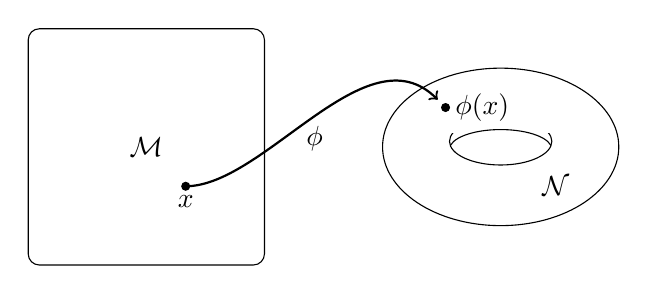
\begin{tikzpicture}
                        \draw[rounded corners](0,0) rectangle (3,3);
                        \node at (1.5,1.5) {\(\mathcal{M}\)};
                        \draw[fill](2,1) circle (0.05) node[below] {\(x\)};

                        \draw(6,1.5) ellipse (1.5 and 1);
                        \begin{scope}
                            \clip(6,1.57) ellipse (0.65 and 0.3);
                            \draw(6,1.47) ellipse (0.65 and 0.25);
                        \end{scope}
                        \begin{scope}
                            \clip(4.5,0) rectangle (7.5,1.67);
                            \draw(6,1.57) ellipse (0.65 and 0.3);
                        \end{scope}
                        \draw[fill](5.3,2) circle (0.05) node[right] {\(\phi(x)\)};
                        \node at (6.7,1) {\(\mathcal{N}\)};

                        \draw[thick,->](2,1) .. controls (3,1) and (4.3,3) .. (5.2,2.1) node[midway, below] {\(\phi\)};
                    \end{tikzpicture}
                \end{figure}
            \item \(\psi\) a (Dirac) spinor on \(\mathcal{M}\).
            \item Gauge fields \(A_\mu(x)\) (taking values in \(\Omega^1(\mathcal{M},\mathcal{L}(G))\), i.e. the set of all 1-forms on \(\mathcal{M}\) with coefficients in the Lie algebra of some Lie group \(G\)).
        \end{itemize}
    \item We must pick an action \(S:\mathcal{C}\rightarrow\RR\), where \(\mathcal{C}\) is the space of fields. For example:
        \begin{itemize}
            \item For a scalar field \(\phi\):
                \begin{equation}
                    S[\phi] = \int_\mathcal{M}\dd[d]{x}\sqrt{g}\Big[ \underbrace{\frac{g^{\mu\nu}}{2}\partial_\mu\phi\partial_\nu\phi}_{\text{kinetic term}}-\underbrace{V(\phi)}_{\mathclap{\substack{\text{potential}\\\text{term}}}} \Big]
                \end{equation}
            \item For a gauge field \(A\):
                \begin{equation}
                    S[A] = \frac{1}{4e^2}\int\dd[d]{x}\sqrt{g}g^{\mu\nu}g^{\rho\sigma}\underbrace{(F_{\mu\rho},F_{\nu\sigma})}_{\text{Killing form}}
                \end{equation}
        \end{itemize}
        In general, the action, even for a scalar, can be the integral of an arbitrary differential polynomial in the fields:
        \begin{equation}
            S[\phi] = \int \underbrace{\mathcal{L}(\phi,\partial^p\phi)}_{\mathclap{\substack{\text{polynomial in }\phi\\\text{and all derivatives}}}} \sqrt{g} \dd[d]{x}
        \end{equation}
\end{enumerate}

\section{QFT in zero dimensions}
If \(\dim \mathcal{M} = 0\) and \(\mathcal{M}\) is connected, then \(\mathcal{M}=\{\text{pt}\}\). We'll choose our fields to be \(\phi:\{\text{pt}\}\rightarrow\RR\) (i.e. \(\phi\in\RR\)).

The basic object we want to compute (in any QFT) is the partition function:
\begin{equation}
    Z = \int_\mathcal{C} \Dd{\phi} e^{-S[\phi]}
\end{equation}
which in this case is just:
\begin{equation}
    Z = \int_\RR \dd{\phi} e^{-S(\phi)}
\end{equation}
We'll assume that \(e^{-S(\phi)}\) decays sufficiently rapidly as \(|\phi|\rightarrow\infty\) that this integral converges. In practice, we take \(S(\phi)\) to be an even degree polynomial in \(\phi\), for example:
\begin{equation}
    S(\phi) = \frac{m^2}{2}\phi^2 + \frac{\lambda}{4!}\phi^4
\end{equation}
In this case \(Z=Z(m,\lambda,\dots)\) is a function of all the coupling constants in \(S(\phi)\). For example:
\begin{equation}
    Z(m^2) = \int_\RR \dd{\phi}e^{-m^2\phi^2/2} = \frac{\sqrt{2\pi}}{m}
\end{equation}
If we include more terms, integrals become hard to solve:
\begin{equation}
    Z(m^2,\phi) = \int_\RR e^{-m^2\phi^2/2-\lambda\phi^4/4!}
\end{equation}
We can try to evaluate this perturbatively in \(\lambda\):
\begin{align}
    Z(m^2,\phi) &= \int \dd{\phi} \left( e^{-m^2\phi^2/2} \sum_{n=0}^\infty \left( \frac{-\lambda}{4!} \right)^n\frac{\phi^{4n}}{n!} \right)\\
    &\stackrel{?}{\sim} \sum_{n=0}^\infty \left( \frac{-\lambda}{4!} \right)^n\frac{1}{n!}\int\dd{\phi}\phi^{4n}e^{-m^2\phi^2/2}
\end{align}
This integral can't possibly converge as a power series in \(\lambda\). In fact this is an asymptotic series\footnote{
    Recall: \(\sum_{n=0}^\infty a_n\lambda^n\) is an asymptotic series for \(Z(\lambda)\) if:
    \begin{equation}
        \lim_{\lambda\rightarrow 0} \frac{|Z(\lambda)-\sum_{n=0}^Na_n\lambda^n|}{\lambda^N}=0 \quad \text{for all } N\in\NN
    \end{equation}
} for \(Z(m^2,\lambda)\). Feynman diagram expansions in QFT are (almost) always asymptotic expansions. It can be shown :
\begin{align}
    Z(m^2\lambda) &\sim \frac{\sqrt{2\pi}}{m}\left[ 1-\frac{\lambda}{8m^4} + \frac{35}{384}\frac{\lambda^2}{m^4} + \dots \right]
\end{align}
Inductively, the coefficient of \(\lambda^n\) is \(\frac{1}{(4!)^nn!}\times\frac{(4n)!}{4^n(2n)!}\). We expect \(\frac{1}{(4!)^nn!}\) as the coefficient in a series expansion. \(\frac{(4n)!}{4^n(2n)!}\) is the number of ways of joining \(4n\) objects into pairs.

\subsection{Feynman rules}
\lecture{18/01/16}
We represent each term in the asymptotic series as a graph. Each propagator %
\raisebox{.2\baselineskip}{\begin{tikzpicture}
    \draw (0,0) -- (1,0);
\end{tikzpicture}} %
contributes a factor of \(\frac{1}{m^2}\), and each vertex %
\raisebox{-.5\height+.2\baselineskip}{
\begin{tikzpicture}[scale=0.3]
    \draw (0,0) -- (1,1);
    \draw (1,0) -- (0,1);
    \fill (0.5,0.5) circle (0.15);
\end{tikzpicture}} %
contributes a factor of \(-\lambda\). For the partition function, we just want vacuum graphs, so we have no external legs. Feynman rules tell us to draw all such graphs, imagining that the lines emanating from each vertex are labelled. For example, at first order (one vertex), we can make the following graphs:
\begin{figure}[H]
    \centering
    \begin{tikzpicture}
        \draw[thick,->] (-3.2,0) -- (-2.3,0);
        \begin{scope}[shift={(-4.5,0)}]
            \draw (-0.5,-0.5) -- (0.5,0.5);
            \draw (-0.5,0.5) -- (0.5,-0.5);
            \fill (0,0) circle (0.05);
            \node[above] at (0.5,0.5) {1};
            \node[below] at (0.5,-0.5) {2};
            \node[below] at (-0.5,-0.5) {3};
            \node[above] at (-0.5,0.5) {4};
        \end{scope}
        \begin{scope}[shift={(7,0)}]
            \draw (0,0) arc (135:-225:1);
            \fill[white] ({sqrt(2)},0) circle (0.1);
            \draw (0,0) arc (225:-135:1);
            \fill (0,0) circle (0.05);
            \node[above] at (0.5,0.3) {1};
            \node[below] at (0.5,-0.3) {2};
            \node[left] at (-0.3,-0.5) {3};
            \node[left] at (-0.3,0.5) {4};
        \end{scope}
        \begin{scope}[shift={(3.5,0)},rotate=-90]
            \draw (0,0) .. controls (2,2) and (2,-2) .. (0,0)
                        .. controls (-2,2) and (-2,-2) .. cycle;
            \fill (0,0) circle (0.05);
            \node[right] at (-0.5,0.5) {1};
            \node[right] at (0.5,0.5) {2};
            \node[left] at (0.5,-0.5) {3};
            \node[left] at (-0.5,-0.5) {4};
        \end{scope}
        \begin{scope}
            \draw (0,0) .. controls (2,2) and (2,-2) .. (0,0)
                        .. controls (-2,2) and (-2,-2) .. cycle;
            \fill (0,0) circle (0.05);
            \node[above] at (0.5,0.5) {1};
            \node[below] at (0.5,-0.5) {2};
            \node[below] at (-0.5,-0.5) {3};
            \node[above] at (-0.5,0.5) {4};
        \end{scope}
    \end{tikzpicture}
\end{figure}
Hence, the first order term in the expansion is given by:
\begin{figure}[H]
    \centering
    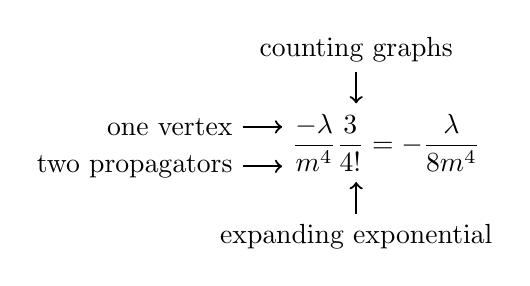
\begin{tikzpicture}
        \node[right] at (0,0) {\(\displaystyle\frac{-\lambda}{m^4}\frac{3}{4!} = - \frac{\lambda}{8m^4}\)};

        \draw[thick,<-] (0,0.2) -- (-0.5,0.2) node[left] {one vertex};
        \draw[thick,<-] (0,-0.3) -- (-0.5,-0.3) node[left] {two propagators};
        \draw[thick,<-] (0.94,0.5) -- (0.94,0.9) node[above] {counting graphs};
        \draw[thick,<-] (0.94,-0.5) -- (0.94,-0.9) node[below] {expanding exponential};
    \end{tikzpicture}
\end{figure}
Drawing \emph{all} of these graphs can be very laborious. There is a shortcut.

Let \(D_n\) be the set of all labelled graphs with \(n\) vertices. Each will come with a factor of \(-\lambda^n\), but as topological (i.e. unlabelled) graphs, we've overcounted, and we should account for this. \(D_n\) is naturally acted on by the group \((S_4)^n\times S_n\), where the \(S_4\)s act by permuting the labels at each vertex, and the \(S_n\) acts be permuting the vertices themselves. This group has order \((4!)^nn!\) and so the weight of Feynman graphs with
\(n\) vertices is \(|D_n|/(4!)^nn!\).

It's useful to rewrite this in the following way. Let \(\Gamma\) be an orbit of \(G_n=(S_4)^n\times S_n\) in \(D_n\), i.e. \(\Gamma\) is a topologically distinct unlabelled graph. As an example, the following two graphs are distinct:
\begin{figure}[H]
    \centering
    \begin{tikzpicture}
        \begin{scope}
            \draw (0,0) .. controls (1,0.9) and (2,0.9) .. (3,0);
            \draw (0,0) .. controls (1,0.3) and (2,0.3) .. (3,0);
            \draw (0,0) .. controls (1,-0.3) and (2,-0.3) .. (3,0);
            \draw (0,0) .. controls (1,-0.9) and (2,-0.9) .. (3,0);
            \fill (0,0) circle (0.05);
            \fill (3,0) circle (0.05);
        \end{scope}
        \node at (4.3,0) {\(\not\sim\)};
        \begin{scope}[shift={(6,0)}]
            \fill (1,0) circle (0.05);
            \fill (4,0) circle (0.05);
            \draw (1,0) .. controls (2,1) and (3,1) .. (4,0) 
                        .. controls (6,-2) and (6,2) .. (4,0)
                        .. controls (3,-1) and (2,-1) .. (1,0)
                        .. controls (-1,2) and (-1,-2) .. cycle;
        \end{scope}
    \end{tikzpicture}
\end{figure}
Also, let \(\mathcal{O}_n\) be the set of these orbits (i.e. the set of topologically distinct graphs with \(n\) vertices). Then the orbit-stabilizer theorem states that:
\begin{equation}
    \frac{|D_n|}{|G_n|} = \sum_{\Gamma\in\mathcal{O}_n}\frac{1}{|\text{Aut}\,\Gamma|}
\end{equation}
where \(\text{Aut}\,\Gamma\) is the set of elements in \(G_n\) that fix \(\Gamma\). \(|\text{Aut}\,\Gamma|\) is sometimes called the \emph{symmetry factor}.

Thus the weight of the \(n\) vertex contribution to the asymptotic series for \(Z(m,\lambda)\) is:
\begin{equation}
    \frac{(-\lambda)^n}{m^{4n}}\sum_{\Gamma\in\mathcal{O}_n}\frac{1}{|\text{Aut}\,\Gamma|}
\end{equation}
and therefore we have:
\begin{align}
    \frac{Z(m,\lambda)}{Z(m,0)} &= \sum_{n=0}^\infty \left( \frac{(-\lambda)^n}{m^{4n}}\sum_{\Gamma\in\mathcal{O}_n}\frac{1}{|\text{Aut}\,\Gamma|} \right) \\
    &= \sum_\Gamma \frac{1}{|\text{Aut}\,\Gamma|} \frac{(-\lambda)^{|v(\Gamma)|}}{(m^2)^{|e(\Gamma)|}}
\end{align}
where \(|e(\Gamma)|\) is the number of edges, and \(|v(\Gamma)|\) is the number of vertices.

As a sanity check, lets use this to calculate the first few terms:
\begin{figure}[H]
    \centering
    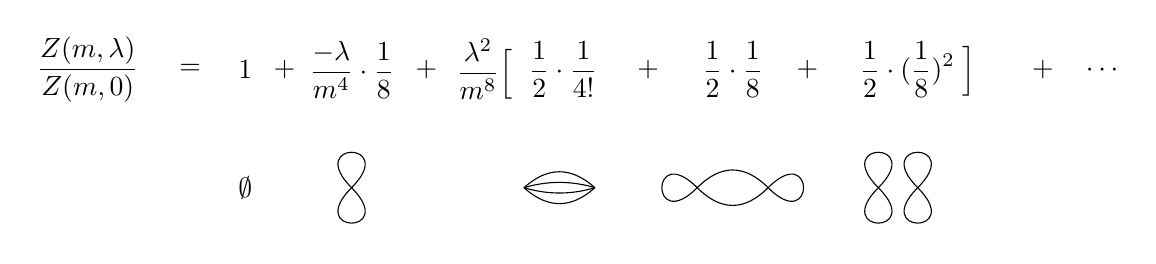
\begin{tikzpicture}
        \node at (0,0) {\(\displaystyle \frac{Z(m,\lambda)}{Z(m,0)}\)};
        \node at (1.3,0) {\(=\)};

        \begin{scope}[shift={(2,0)}]
            \node at (0,0) {1};
            \node at (0,-1.5) {\(\emptyset\)};
        \end{scope}
        \node at (2.5,0) {\(+\)};
        \begin{scope}[shift={(3.35,-1.5)}]
            \draw[rotate=90, scale=0.3] (0,0) .. controls (2,2) and (2,-2) .. (0,0)
                        .. controls (-2,2) and (-2,-2) .. cycle;
            \node at (0,1.5) {\(\displaystyle \frac{-\lambda}{m^4}\cdot\frac{1}{8}\)};
        \end{scope}
        \node at (4.3,0) {\(+\)};
        \begin{scope}[shift={(5.04,0)}]
            \begin{scope}[shift={(0.5,-1.5)},scale=0.3]
                \draw (0,0) .. controls (1,0.9) and (2,0.9) .. (3,0);
                \draw (0,0) .. controls (1,0.3) and (2,0.3) .. (3,0);
                \draw (0,0) .. controls (1,-0.3) and (2,-0.3) .. (3,0);
                \draw (0,0) .. controls (1,-0.9) and (2,-0.9) .. (3,0);
            \end{scope}
            \begin{scope}[shift={(2.4,-1.5)}]
                \draw[scale=0.3] (1,0) .. controls (2,1) and (3,1) .. (4,0) 
                            .. controls (6,-2) and (6,2) .. (4,0)
                            .. controls (3,-1) and (2,-1) .. (1,0)
                            .. controls (-1,2) and (-1,-2) .. cycle;
            \end{scope}
            \begin{scope}[shift={(5,-1.5)}]
                \draw[rotate=90, scale=0.3] (0,0) .. controls (2,2) and (2,-2) .. (0,0)
                            .. controls (-2,2) and (-2,-2) .. cycle;
            \end{scope}
            \begin{scope}[shift={(5.5,-1.5)}]
                \draw[rotate=90, scale=0.3] (0,0) .. controls (2,2) and (2,-2) .. (0,0)
                            .. controls (-2,2) and (-2,-2) .. cycle;
            \end{scope}
            \node at (0,0) {\(\displaystyle\frac{\lambda^2}{m^8}\Big[\)};
            \node at (1,0) {\(\displaystyle\frac{1}{2}\cdot\frac{1}{4!}\)};
            \node at (2.075,0) {\(+\)};
            \node at (3.15,0) {\(\displaystyle\frac{1}{2}\cdot\frac{1}{8}\)};
            \node at (4.1,0) {\(+\)};
            \node at (5.5,0) {\(\displaystyle\frac{1}{2}\cdot\qty(\frac{1}{8})^2\;\Big]\)};
            \node at (7.5,0) {\(+\quad\cdots\)};
        \end{scope}
    \end{tikzpicture}
\end{figure}
which if we do the arithmetic will lead to agreement with the above.

More generally we may have several types of field \(\phi_i\), each with some propagator \(\frac{1}{P_i}\). These may interact through many types of vertices \(\alpha\), each with coupling constant \(\lambda_\alpha\). Then the partition function has an asymptotic series expansion:
\begin{align}
    \frac{Z}{Z|_{\lambda_\alpha=0}} &= 
    \sum_\Gamma \frac{1}{|\text{Aut}\,\Gamma|}\frac{\prod_\alpha(-\lambda_\alpha)^{|v_\alpha(\Gamma)|}}{\prod_i P_i^{|e_i(\Gamma)|}} \\
    &= \exp \qty( \sum_{\Gamma\text{ connected}} \frac{1}{|\text{Aut}\,\Gamma|}\frac{\prod_\alpha(-\lambda_\alpha)^{|v_\alpha(\Gamma)|}}{\prod_i P_i^{|e_i(\Gamma)|}} ) \\
    &= \exp(W)
\end{align}
where we use the last line to define \(W\), the (Helmholtz) free energy.

\subsection{Schwinger-Dyson equations}
Trivially, \(Z = \int_\RR\dd{\phi}e^{-S(\phi)} = \int_\RR\dd{(\phi+\epsilon)}e^{-S(\phi+\epsilon)}\) for any constant \(\epsilon\). By translational invariance of the measure, \(\dd{(\phi+\epsilon)} = \dd{\phi}\), so we have:
\begin{equation}
    Z = \int_\RR\dd{\phi}e^{-S(\phi+\epsilon)} = \int_\RR\dd{\phi}e^{-S(\phi)}\left[ 1 - \epsilon\pdv{S}{\phi} \right] + O(\epsilon^2)
\end{equation}
If we compare this to our original expression for \(Z\), we see \(Z = Z - \epsilon\int\dd{\phi}e^{-S}\pdv{S}{\phi}+O(\epsilon^2)\), which implies:
\begin{equation}
    \expval{\pdv{S}{\phi}} = 0
\end{equation}
where we take the normal definition of the expectation of a function \(f(\phi)\) for a given partition function:
\begin{equation}
    \expval{f(\phi)} = \frac{1}{Z}\int\dd{\phi}e^{-S(\phi)}f(\phi)
\end{equation}
This is essentially Ehrenfest's theorem: the expectation value of the classical equation of motion holds. For example, if \(S=\frac{m^2\phi^2}{2} + \frac{\lambda\phi^4}{4!}\), then we have \(\expval{\pdv{S}{\phi}} = \expval{m^2\phi+\frac{\lambda\phi^3}{3!}} = 0\).

\end{document}
